1 in 14 children in the U.S. has a speech or language disorder, such as dyslexia or Autism, that can hinder reading, vocabulary growth, and communication~\cite{nidcd2023, cde2024, crossriver2024, gorno2011classification-ppa}. These delays can affect quality of life, academic success, and future opportunities. Thus, developing a reliable and automatic framework for evaluating kids language function, covering verbal skills, developmental milestones, reading, and comprehension, is essential. It enables early detection of delays and supports educators and specialists in early identification and intervention.


The bottleneck in developing such a framework lies in the accurate transcription of kids speech, which is significantly more challenging than that of adults. This difficulty arises from several unique characteristics of child vocalizations, including higher fundamental frequency, longer phone durations, greater articulatory variability, and persistent data sparsity~\cite{lee1997analysis, tran2020analysis, neuberger2014cross, gerosa2009review, yeung2018difficulties, shankar2025selective}. 

Although recent work has produced increasingly robust child-oriented Automatic Speech Recognition (ASR) models~\cite{fan2024benchmarking, bhardwaj2022automatic, shahnawazuddin2024developing, singh2025causal, singh2021data, kathania2022formant, fan2022towards, xu24c_interspeech, kim2021conditionalvariationalautoencoderadversarial}, most developmentally significant pronunciation errors arise at the sub-word level and are consequently hidden by word-level metrics such as Word Error Rate (WER). Consider the prompt bird /\textipa{b@rd}/: a child who utters /\textipa{bed}/ (“bed”) exhibits a phoneme substitution, while /\textipa{pb@rd}/ (“p-bird”) contains an intrusive plosive. State-of-the-art end-to-end ASR systems often output the canonical word bird for both productions, masking the underlying articulatory deviation. A dedicated \textit{sub-word recognizer} that reliably recovers phoneme sequences is therefore indispensable for fine-grained kids language function evaluation, where \textit{phoneme recognition} is the most widely used approach.

Traditional work has primarily focused on fine-tuning children's speech data on pretrained self-supervised speech learning (SSL) models~\cite{li2024enhancingchildvocalizationclassification, li2024analysisselfsupervisedspeechmodels, Shi-JASAEL-2024, gao2024g2pu, peng2023study, 10971198, zhu2022phone-w2v2-alignment, zhao-etal-2025-mutis, mohamed2022selfreview, hsu2021hubert, Chen_2022}. However, these approaches exhibit poor generalizability to open-domain children's speech. Moreover, directly adopting adult-oriented ASR or phoneme recognition pipelines fails to address allophonic variations and disrupted phoneme-level language structures. 

Unlike purely data-driven approaches, the real breakthrough in modeling atypical speech transcription lies in the development of disfluent speech transcription pipelines that incorporate human and linguistic priors~\cite{ssdm, zwilling2025speech, ye2025seamlessalignment-neurallcs, zhang2025analysisevaluationsyntheticdata, lian22b_interspeech-gestures, lian2023articulatory-factors}. A state-of-the-art example is Dysfluent Weighted Finite State Transducer (D-WFST), which leverages WFST to model disrupted phoneme structures~\cite{guo2025dysfluentwfstframeworkzeroshot}. However, these WFST-based approaches lack robustness in detecting subtle phonetic variations, particularly substitutions and deletions, an issue especially pronounced in downstream applications involving audio with moderate to severe disfluency.

In this work, we present K-Function, a comprehensive framework for evaluating children’s language function. It consists of our newly proposed Kids-Weighted Finite State Transducer (K-WFST), a lightweight and interpretable kids phoneme transcription model—an LLM-boosted automatic language function scoring system, and a feedback component. Together, these modules form a unified assessment framework for generalized language function evaluation in children.

K-Function is evaluated on two child speech datasets MyST~\cite{ward2011my} and Multitudes~\cite{UCSFMultitudes2025}. Our framework consistently achieves superior phoneme recognition, enables more accurate language function scoring via Large Language Models (LLMs), and aligns closely with real proctor scores.

Crucially, the high-fidelity transcriptions from K-WFST provide the foundation for a complete assessment-feedback loop, powering sophisticated downstream analyses. These results collectively highlight that accurate sub-word recognition is a crucial, missing cornerstone for kids language function evaluation. Our K-Function makes the following key contributions:



\begin{figure*}[h]
\vspace{-2mm}
    \centering
     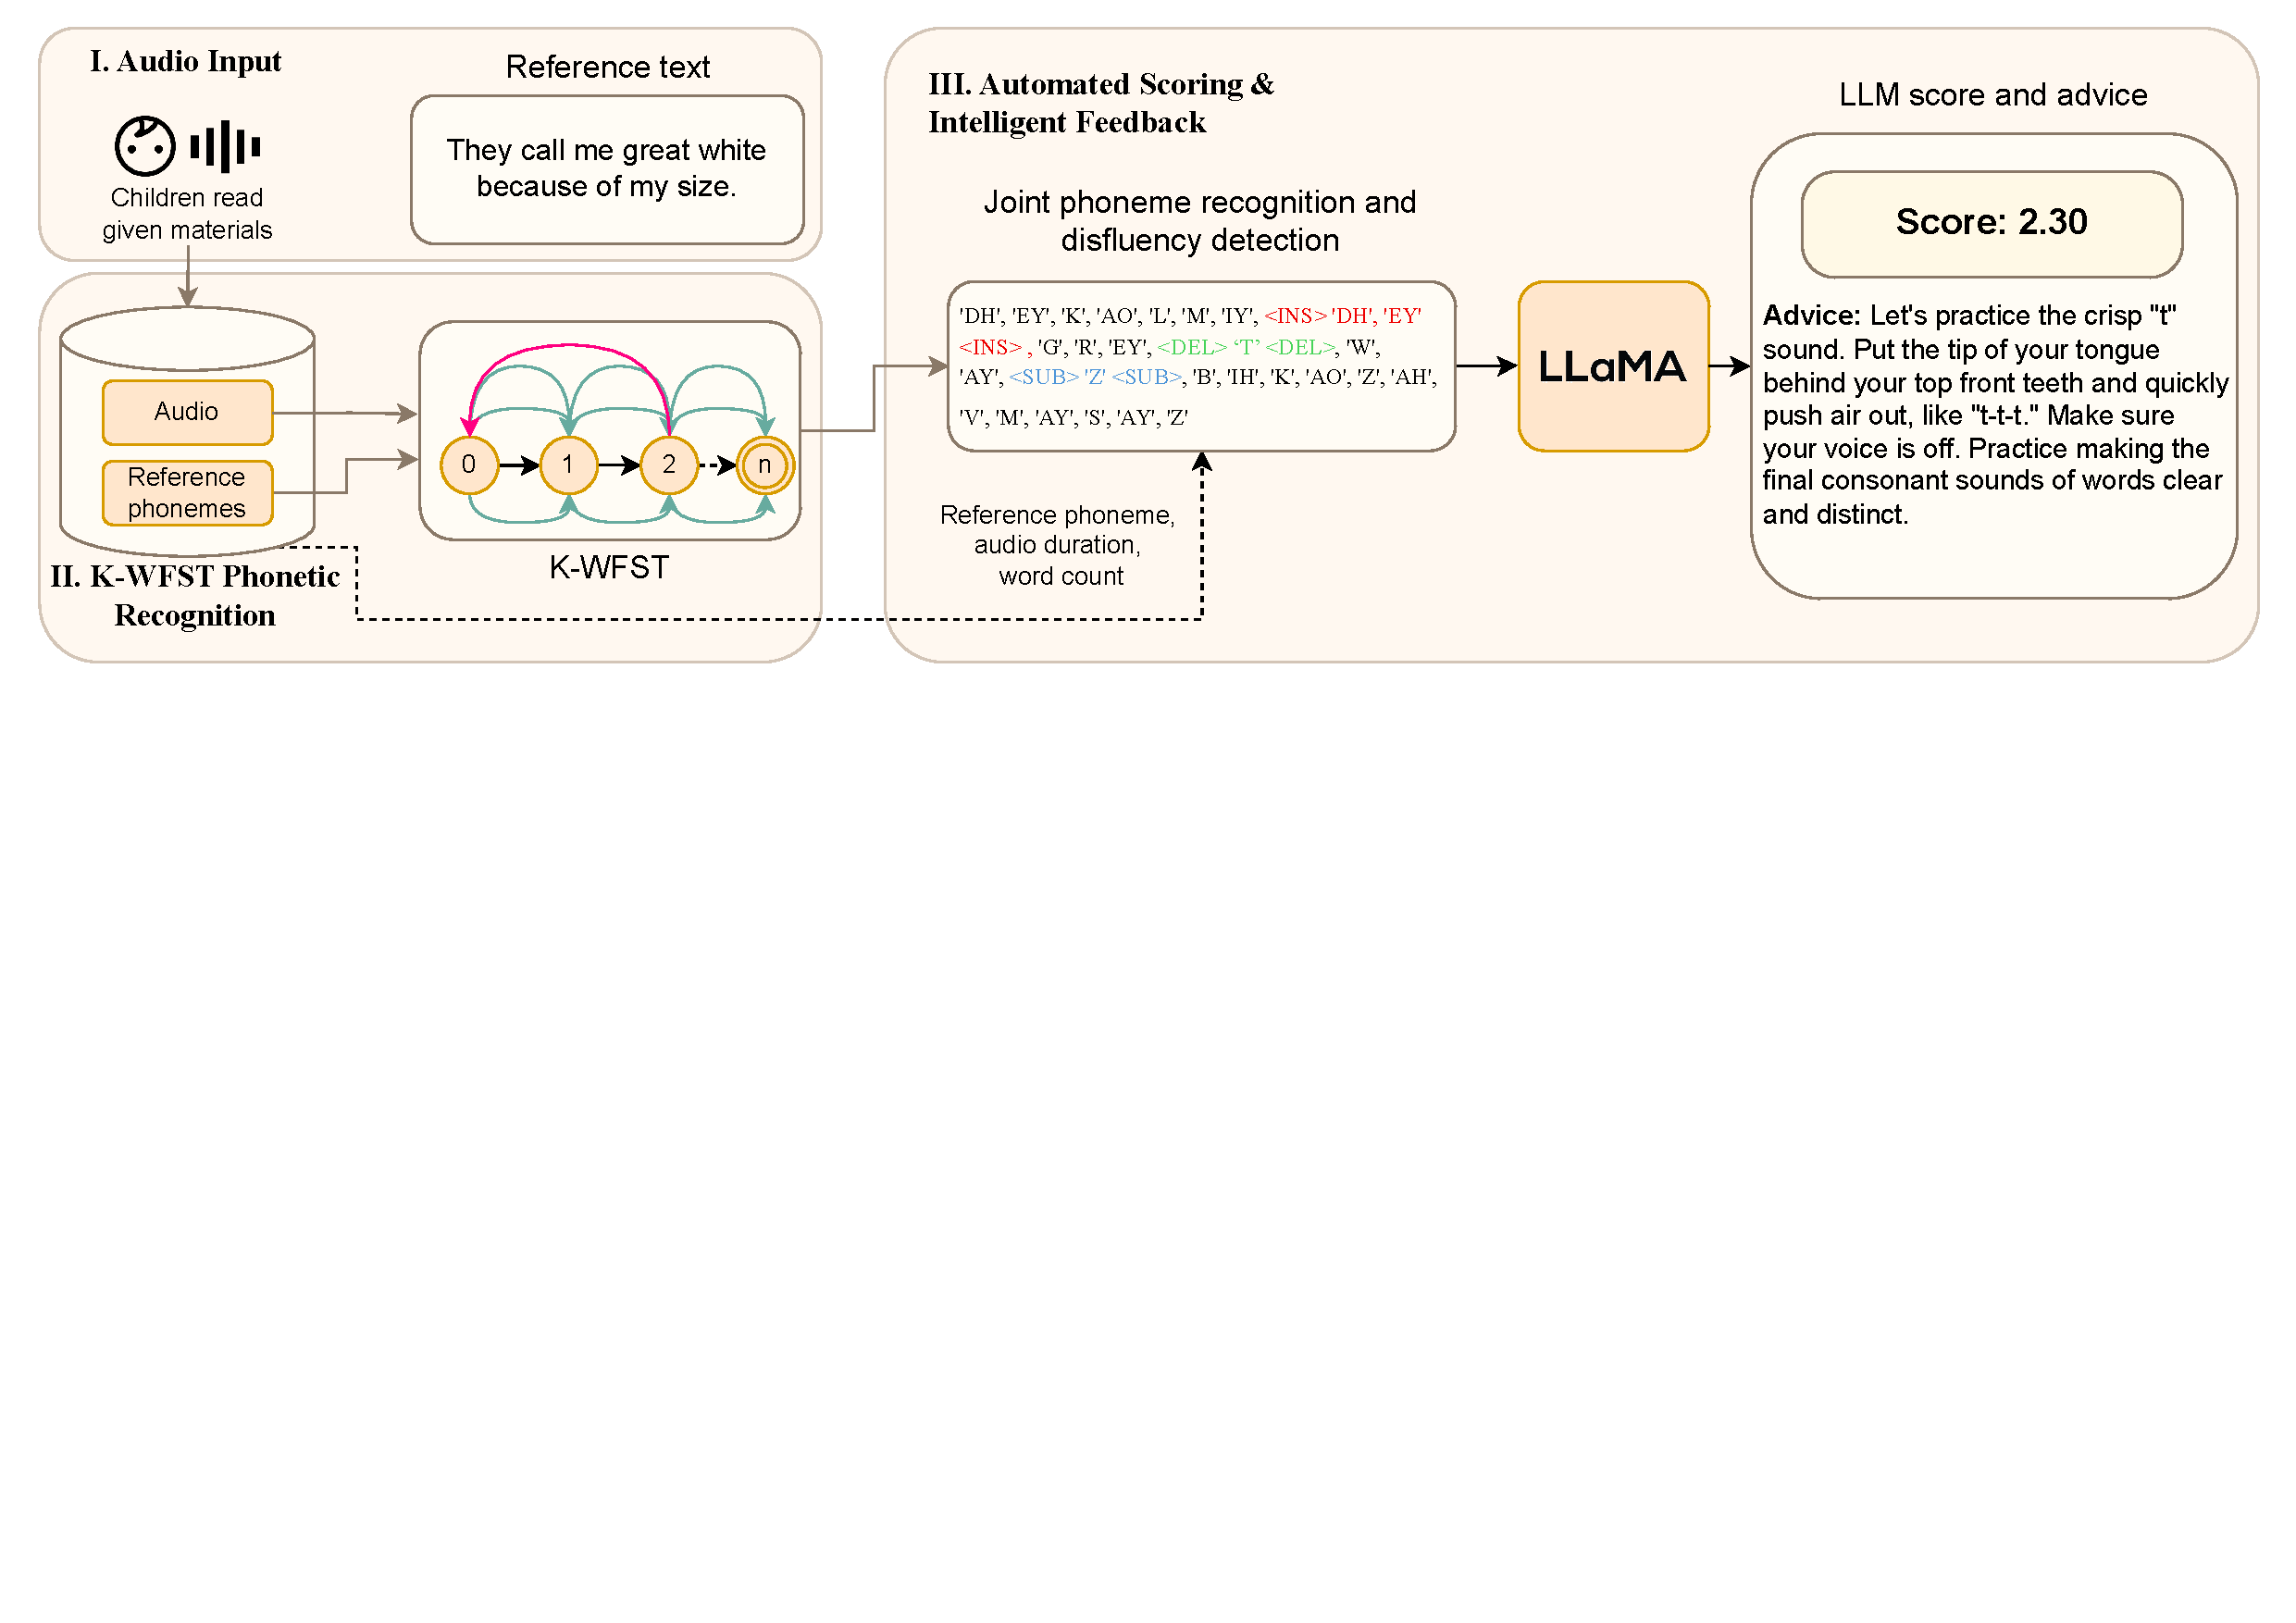
\includegraphics[width=\textwidth]{image/Kids-WFST.pdf}
    \caption{The 3-stage pipeline of the K-Function framework, from audio input to a comprehensive feedback report.}
    \label{fig:pipeline}
\vspace{-5mm}
\end{figure*}

\textit{(1) K-WFST:} We present a WFST decoder designed specifically for children’s speech, which achieves state-of-the-art phoneme error rates (PER) on both the MyST~\cite{ward2011my} and Multitudes~\cite{UCSFMultitudes2025} corpora.

\textit{(2) A Unified Assessment Framework:} We propose a complete system that integrates our state-of-the-art sub-word transcription (K-WFST) with an advanced LLM-based scoring module to create a robust pipeline for automated language function assessment.

\textit{(3) Align with Proctor Scores and Go Beyond:} Our framework's automated scores show high consistency with the manual scores given by expert proctors on the Multitudes corpus. Critically, our system also provides detailed, phoneme-level error analysis, offering insights that are difficult to achieve at scale through manual scoring alone.

\textit{(4) Demonstrated Downstream Utility:} We show significant value in practical applications, including achieving higher consistency in LLM-assisted language function assessment.
